\chapter{実験}
予備実験を含め,行なった実験は9種類ある.

予備実験として,DCADとレスキュー犬訓練データセットの2種類のクラス分類を行なった.

本実験では,
静止画像からのマルチラベル推定,
optical flow画像からのマルチラベル推定,
音声データからのマルチラベル推定2種,
Sound based Two-stream networkを用いた音声データと静止画像からのマルチクラス推定,
同じくSound based Two-stream networkを用いた音声データとoptical flow画像からのマルチクラス推定,
そしてSound based Three-stream networkを用いた音声データと静止画像とoptical flow画像からのマルチクラス推定の7種類を行なった.
\section{予備実験:クラス分類}
DCADとレスキュー犬訓練データセットについて,それぞれクラス分類を行なった.
DCADはクリップ毎にフレーム間の平均をとり,画像として扱ってVGG16のpretrained modelを用いてfinetuningを行なった.
レスキュー犬訓練データセットは動画をラベル毎に切り出して短いクリップ群を作り,そのクリップ毎に同様にフレーム間の平均を取った画像を作成しVGG16のpretrained modelを用いてfinetuningした.
\subsection{DCAD動画像平均画像クラス分類}
予備実験の結果を~(図\ref{vgg16_res}に示す.分類率は64.3\%であった.
全般的に,データの多いクラスは精度が高い傾向にあるが,データの少ないクラスは精度が低い傾向にある.
加えて,~\(Car\)クラスは道路の進行方向に対して垂直に待機している10クラスの中で特殊なクラスであり,車などの写ったフレームの影響で分類精度が上昇していると考えられる.~\(Feed\)クラス,~\(Pet\)クラス,~\(Play\_with\_ball\)クラスは,それぞれフレーム内を人間が占める割合が多いクラスと言え,そのため混同が起こりやすいと考えられる.

\begin{figure}[htbp]
 % \begin{tabular}{cc}
 %  \begin{minipage}{0.5\textwidth}
   \begin{center}

    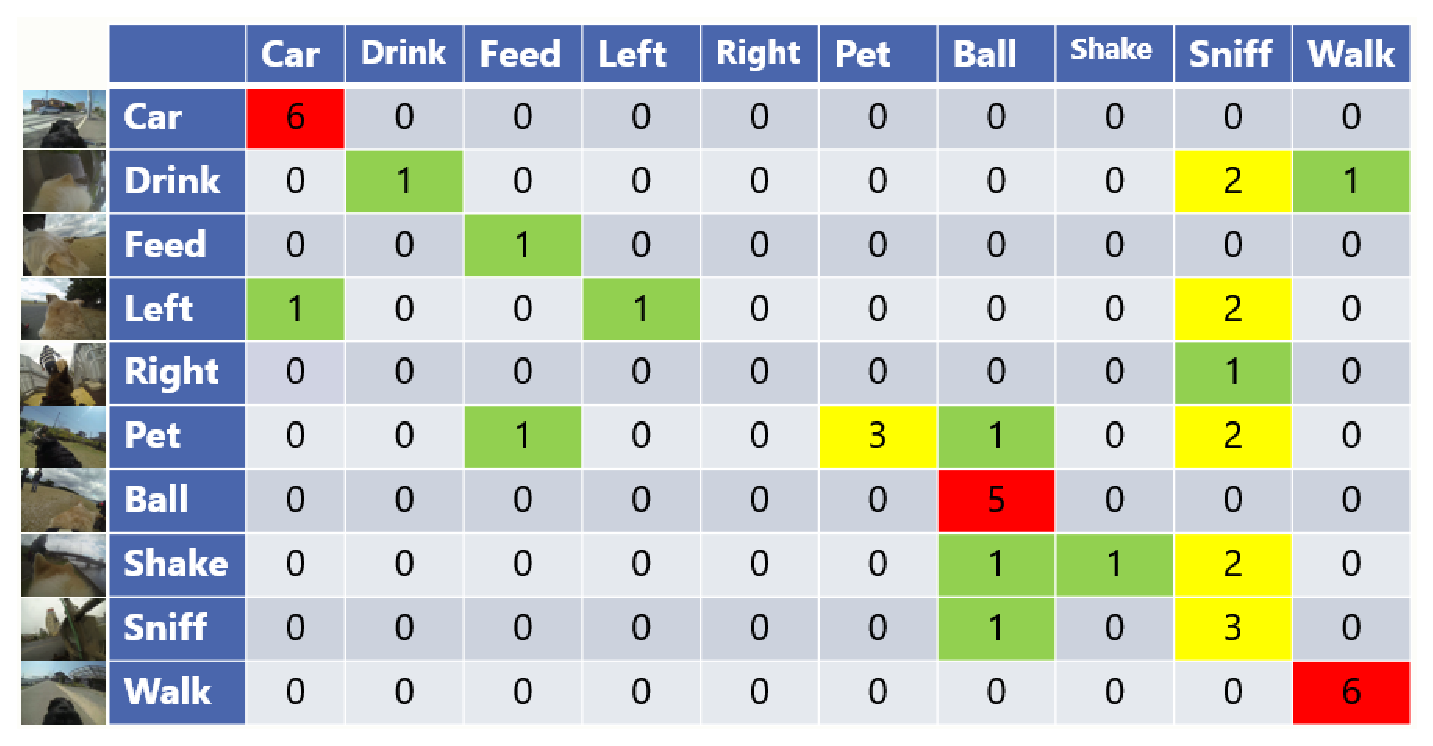
\includegraphics[scale=0.5]{./Figures/vgg16_res.eps}
    \caption{VGG16 pretrained modelによるfinetuningの結果}
    \label{vgg16_res}
   \end{center}
  % \end{minipage}
  % \begin{minipage}{0.5\textwidth}
\end{figure}

%% \subsection{レスキュー犬訓練データセット動画像平均画像クラス分類}
%% \begin{figure}[htbp]

%%    \begin{center}

%%     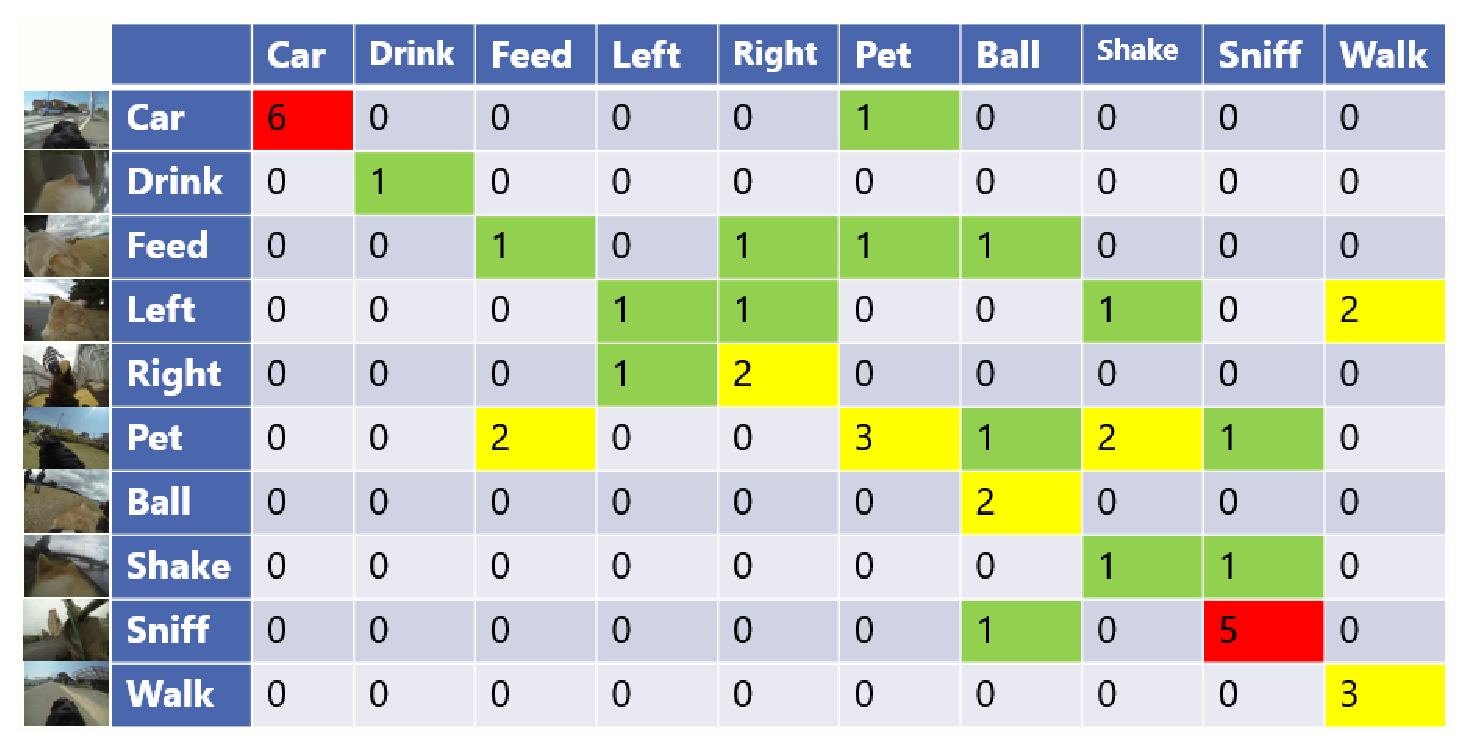
\includegraphics[scale=0.3]{./Figures/resnet_res.eps}
%%   \caption{ResNet pretrained modelによるfinetuningの結果}
%%   \label{resnet_res}
%%    \end{center}
%%  %  \end{minipage}
%%  % \end{tabular}
%% \end{figure}
%\section{オプティカルフロー動画平均画像クラス分類}
%動画像のフレーム間の平均を取った手法と同様に,クリップ毎にoptical flowの平均画像を作成しVGG16のpretrained modelを用いてfinetuningを行なった.
\subsection{レスキュー犬訓練データセット動画像平均画像クラス分類}

